\documentclass{llncs}
%\documentclass{article}
\usepackage[utf8]{inputenc}
\usepackage{cite}
\usepackage{verbatim}
\usepackage{graphicx}
%\usepackage{wrapfig}
\usepackage{appendix}

\newcommand{\rdfterm}[1]{\texttt{#1}}
\newcommand{\pvalue}{\textit{p}-value\ }
\newcommand{\httph}[1]{\texttt{#1}}
\newcommand{\todo}[1]{\ensuremath{^{\textrm{\tiny{TODO}\normalsize}}}\footnote{\textbf{TODO:}~#1}}

\title{A survey of HTTP caching options on the open Semantic Web}
\author{Kjetil Kjernsmo}
\institute{Department of Informatics,
Postboks 1080 Blindern,
N-0316 Oslo, Norway \email{kjetil@kjernsmo.net}}

%\subtitle{---Unpublished Working Draft, do not circulate---}


\begin{document}
\maketitle

\begin{abstract}
Scalability of the data access architecture in the Semantic Web is
dependent on the establishment of caching mechanisms to take the load
off of servers.  Unfortunately, there is a chicken and egg problem
here: Research, implementation, and evaluation of caching
infrastructure is uninteresting as long as data providers do not
publish relevant metadata.  And publishing metadata is useless as long
as there is no infrastructure that uses it.

We show by means of a survey of live RDF data sources that caching
metadata is prevalent enough already to be used in some cases.  On the
other hand, they are not commonly used even on relatively static data,
and when they are given, they are very conservatively set. We point
out future directions and give recommendations for the enhanced use of
caching in the Semantic Web.
\end{abstract}

\section{Introduction}

Caching has been given a prominent place in the foundational documents
of the World Wide Web. Out of the 6 documents that make up the HTTP
1.1 standard, RFC7234 \cite{rfc7234} is entirely devoted to the topic,
and RFC7232 \cite{rfc7232} defines conditional requests, which is also
important when constructing caches. As the former notes:
\begin{quote} 
  The goal of caching in HTTP/1.1 is to significantly improve
  performance by reusing a prior response message to satisfy a current
  request.
\end{quote}
Furthermore, the Architecture of the World Wide Web
\cite{Jacobs:04:AWW} discusses caching throughout, and the definition
of the Representational State Transfer (REST) architectural style
\cite{Fielding_2000_Architectural-Styles} is partly motivated from the
requirement to implement efficient caching. We also note that caching
in the Internet infrastructure, through so-called Content Delivery
Networks, is both a large business area and something that could
provide great value to the Semantic Web.

If used correctly, caching mechanisms will reduce the need to make
HTTP requests, reduce lookups to the backend systems, reduce the need
to make repetitive computations, enable sharing of responses in
Internet infrastructure, improve uptime and reduce latency since
requests may be answered closer to the client.

In spite of this, we have not seen it in widespread use in the
Semantic Web, and therefore we decided to conduct a survey to
investigate the actual compliance to RFC7234 and RFC7232. 
With this paper, we hope to achieve the following:
\begin{enumerate}
\item Understand the actual usage rather than rely on anecdotal
  conceptions.
\item Encourage the implementation of these mechanisms in Semantic Web
  infrastructure.
\item Point out future research directions.
\end{enumerate}

We note that caching is not only useful for long-living information
resources, even though that may be the most important use. If a resource
is frequently requested, it may make sense to cache it even though it
may be fresh for only a very short period.

Caching may be deployed at several different levels: An HTTP cache may
be in a reverse proxy close to the server, in which case it may have
much in common with a conventional database cache. It may also be
anywhere between a server and a client, in which case it may be
shared, i.e. it may cache responses from several servers served to
several clients. Another example is an institutional forward proxy,
which are close to several users. Finally, the User Agent may
implement a private cache for its user at the client side.

As mentioned, two standards are relevant for this study, RFC7234,
which is named ``Caching'' and RFC7232, named ``Conditional
Requests''. The main difference is that the caching standard defines
when a response may be reused without contacting the origin server at
all, whereas the conditional requests define how to validate a
response by contacting the origin server. The two can be combined:
Clients and proxies may use the latter to revalidate a response that
has been cached based on the former.

RFC7234 defines two important headers: \httph{Expires}, whose value is
a date and time of when the response is considered stale, and
therefore should not be used; and \httph{Cache-Control}, which allows
detailed control of the cache, including a \httph{max-age} field,
which gives the time in seconds for how long the the response may be
used from the time of the request. \httph{max-age} takes precedence
over \httph{Expires}. In the following \emph{freshness lifetime} is
understood as the number of seconds that the response may be used
without contacting the origin server. Ideally, the calculation of the
freshness lifetime should be based of the above, we therefore shall
refer to this as ``standards-compliant caching''. However it can also
be based on heuristics, and RFC7234, Section~4.2.2 provides some loose
constraints for such practice, as well as a suggestion for a useful
heuristic. This heuristic is based on a fraction of the time lapsed
between the current time and the modification time given in the
\httph{Last-Modified} header. This approach therefore still requires
the Web server to be cooperative to be successful, but commonly, Web
servers can track this, for example if RDF is served from a file
system, the file modification time is used.

RFC7232, on the other hand, defines a protocol for asking the server
if the cached response is still fresh using conditional requests. This
doesn't burden the content provider with the task of estimating the
time to live beforehand, but then, it must be able to answer if the
resource has changed less expensively than serving the entire
response. Either of two headers must be set by the server to achieve
this: \httph{ETag}, which sets an opaque identifier for the response,
or \httph{Last-Modified} which gives the time and date of the last
modification of the resource. Clients may use these values to retrieve
the updated response only if the resource has changed. Other relevant
headers are described in Table~\ref{tab:headers}
in Appendix~\ref{app:fetcher}.

RFC7234 provides detailed control of caching, and caching may also be
prohibited by the server, either by setting a non-positive freshness
lifetime or explicitly using a \httph{no-store} control field.

In this paper, we study to what extent SPARQL Endpoints, vocabulary
and data publishers support these standards.

\section{Related work}

We are not aware of any surveys of this type. Although the database
literature is rich with query cache literature, it is mostly relevant
to what would happen within the server or between the server and a
reverse proxy, which is opaque to the Internet, and therefore not of
our concern.

The \cite{dyldo2} Dynamic Linked Data Observatory (DyLDO) performed,
and continues to do so, monitoring of parts of the Linked Open Data
Cloud to determine dynamicity characteristics of Linked Data. Caching
is one of their motivations, but they have not published statistics on
HTTP headers.

Linked Data Fragments is claimed in \cite{ldf1} to take advantage of
caching and contrasts this with the unavailability of SPARQL query
caches, and it is claimed that this is an architectural problem.

In \cite{sparqlproxy} the authors implemented a reverse proxy that
controlled the changes to the dataset, and therefore could make sure
the proxy had all the information needed to determine freshness. We
are interested in the situation where the changes cannot be
controlled.

In \cite{umbrich2012hybrid}, the term caching was used in a different
sense than we do, they rather prefetched an entire dataset to a local
store and based on heuristics tried to determine which parts of the
query should be evaluated remotely and locally. \cite{lampo2011cache}
explored when caching had a positive effect on complex SPARQL
queries.

In the broader Web literature, \cite{ager2010revisiting} analysed the
value of caching based anonymized traces of actual Web usage at a
major Internet Service Provider. They find that while caching often
yields little benefit when content is user-generated, they still find
some potential.

While these studies have little overlap with the present paper, they
underline the importance of understanding the current deployment and
future potential. In some of the related work, it is shown that
caching does not necessarily give tangible benefits. Yet, we shall
assume that sharing the meta data required for caching outside of the
server is desirable, and that it is possible in most cases. We shall
see that it most likely will be beneficial in cases that do not
benefit from caching today.

\section{Methodology}
We want to find information resources on the Web, and examine HTTP
headers that may allow caching. To do this, we perform GET requests on
SPARQL endpoints, vocabularies, dataset descriptions and other
resources and record headers recommended by current standards, as well
as obsoleted and non-standard headers. Additionally, we examine the
triples in the returned information resources to see if there is
information there that may be used to calculate heuristic freshness.

We make several approaches to ensure that we visit a large and
representative section of the open Semantic Web. We take SPARQL
Endpoints from the SPARQLES survey \cite{buil2013sparql}, vocabularies
from Linked Open Vocabularies (LOV) \cite{lov2} and prefix.cc, and
we augment these data with spidered data from the Billion Triple
Challenge 2014 \cite{btc-2014} dataset.

We used SPARQLES survey list of SPARQL endpoints as of 2014-11-17, and
filtered out those deemed unresponsive by them. This resulted in a
list of 312 endpoints.

To examine as many different implementations and hosts as possible, we
noted that the Billion Triple Challenge 2014 \cite{btc-2014} dataset
consisted of a 4~GTriple corpus of spidered Web data. To compile a
list of candidates to further examine, we performed a
series of data reduction steps, manually inspecting the result between
each step. The details of this process is given in
Appendix~\ref{app:reduction}.

The end result of this process is a list of 3117 unique hosts, for
each several resources would be visited, some several times, as they
may host SPARQL Endpoints, vocabularies, or other information
resources, by a spider detailed in Appendix~\ref{app:fetcher},
resulting in 7745 requests, done on 2015-01-02. Although this is not a
very large number, we assume that caching headers are usually set on a
per-host basis, and so the number of hosts is more important than the
number of resources.

This results in an NQuads file per host, which is then loaded into a
Virtuoso-based SPARQL Endpoint for analysis by using the statistics
system R\cite{kn:r} in the following section.

\section{Analysis}

\subsection{Different server implementations}

First, we investigated whether certain server implementations provided better support
for caching than others. To do this, we formulated SPARQL queries to
examine the \httph{Server} headers of successful responses, with
optional clauses matching the standard-compliant computed freshness
lifetime (which is the ideal) as well as whether the response had other
features that may assist caching such as modification time,
certain predicates, etc.\todo{promising}

For each unique \httph{Server} header, we found the ones where
\emph{all} responses had a freshness time or a promising feature. For
the former, this amounted to 22 servers. 70 servers always responded
with promising features. Inspecting the values we find the well-known
Virtuoso and Callimachus servers, as well as the Perl modules
RDF::LinkedData and RDF::Endpoint, which is partly developed by and
runs on a server operated by this author. Apart from those, a typical
server string is e.g. \httph{Apache/2.2.22 (Fedora)}, which reveals
very little about the RDF-specific parts of the underlying server
implementation. A quick inspection of all \httph{Server} headers
confirmed that few reveal any further detail.

For a more systematic approach, we wish to test the hypothesis that
some servers are better configured to support caching than others.
Using the methodology given in Appendix~\ref{app:stats}, we find in
both the cases of standard-compliant freshness time and for the other
promising features, the test reports \pvalue = 0.0001. We can conclude
that it is highly likely that some servers are better at exposing
cache headers than others. Unfortunately, since most \httph{Server}
headers only contain generic values, little can be learnt about these
implementations. We note, however, that DBPedia exposes
standards-compliant freshness time of 604800 seconds (i.e. 1 week) for
both LOD and SPARQL endpoints.

\subsection{Other caching headers}

As shown in Table~\ref{tab:headers}, there are also other caching
headers than those mentioned in the introduction. We found
\httph{Pragma} (archaic HTTP 1.0 header) in 287 responses, but except
for two hosts, where they were superfluous, they were only used to
prohibit caching. \httph{Surrogates} were not observed.

\subsection{Distribution of freshness lifetime}

We obtained a successful response from a total 2965 information
resources, either with SPARQL results or RDF data. A successful
response is rather strictly defined, not only must there be a
successful HTTP response after redirects are resolved, the response
must also return a valid RDF media type (unless it is a SPARQL result)
and the response must parse into an RDF model. We have given priority
to survey many hosts since configuration usually doesn't differ much
across a host, especially since it also captures different types of
resources. It is therefore acceptable that the number of resources is
relatively small.

Since we are interested in the properties of valid response, including
examining some of the RDF contained in them, and that web servers may
be configured to instruct clients and proxies to cache errors
differently, we will study the statistical properties of valid
responses.

\subsubsection{Standards-compliant caching headers}

Of the 2965 resources, 405 returned valid headers, but 114 did so to
prohibit caching of the response, and 3 contained conflicting
headers, i.e. set an freshness lifetime, but also prohibited
caching. In most cases, \httph{Cache-Control} and \httph{Expires} both
occurred, but the former is more common than the latter in the cases
where only one of them occur.  Additionally, 269 resources had a
\httph{Cache-Control} header to control other aspects of caching than
lifetime, i.e. to say that only private caches may use the response,
that the cache must be revalidated, or to prohibit caching. 
Note that the freshness lifetime is 0 whenever caching is prohibited.

In Figure~\ref{fig:hardall}, there is a barplot where
the freshness lifetime is grouped in bins. We see that in these
categories, the most common is to prohibit caching. Nevertheless, many
also declare a standards compliant freshness lifetime in minutes to
days.

\begin{figure}[ht]
  \centerline{%
    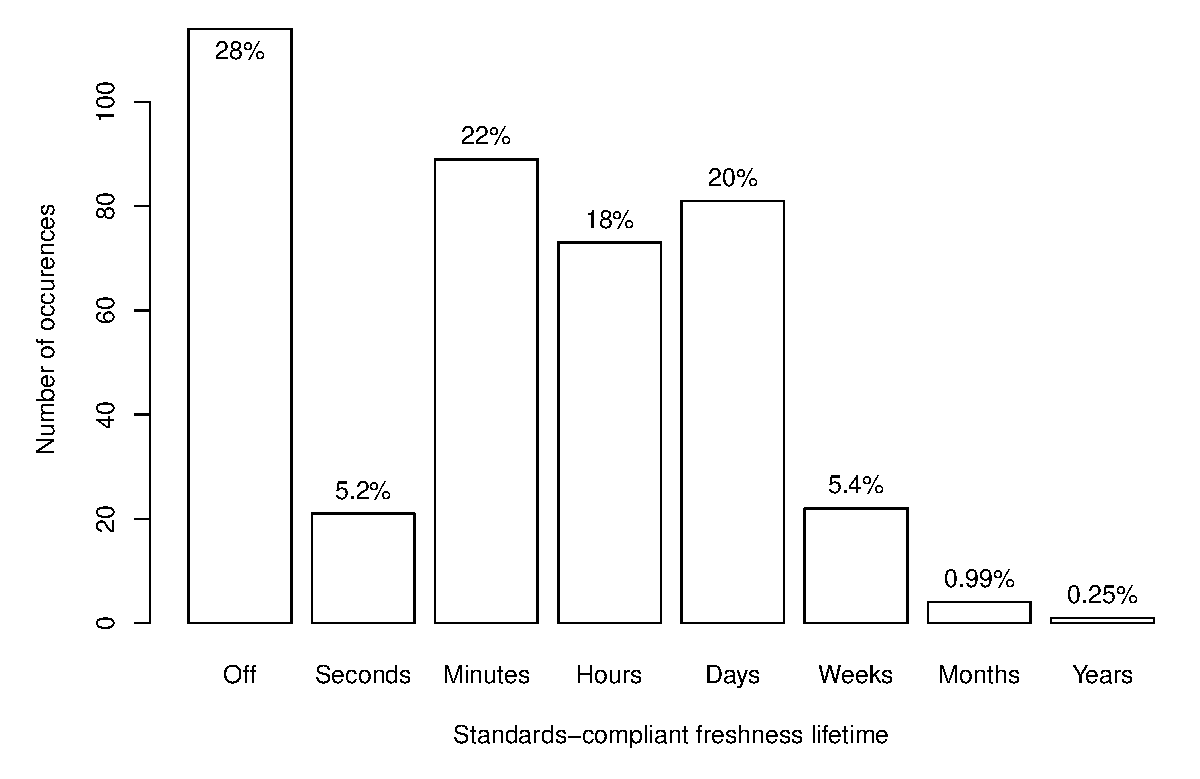
\includegraphics[width=.9\textwidth]{hardall.pdf}}
  \caption{Barplot counting all standard-compliant freshness lifetimes
    found, with the percentage of occurances indicated on the
    bars. The first bin are the cases where caching is explicitly
    prohibited. The next bins are for lifetimes, where the values are
    grouped if they are on the order of seconds, minutes, hours, etc,
    i.e. the second bin counts the lifetimes in the interval [1,59]
    seconds, etc.}
  \label{fig:hardall}
\end{figure}



In Figure~\ref{fig:hardtable}, we have broken this
up by the type of resource that was accessed, i.e. SPARQL endpoints,
vocabularies, dataset descriptions or unclassified information
resources. First, we note that it seems like the distribution of
freshness lifetime is quite different for the different types, an
observation that is also supported by a similar hypothesis test as
above, with a \pvalue = 0.00001. We also note that it is often
prohibited to cache dataset descriptions. This is odd, since
statistics about datasets is usually costly to compute and should be
cached. The VoID specification \cite{voidnote} also notes that the
statistics are considered estimates.

\begin{figure}[ht]
  \centerline{%
    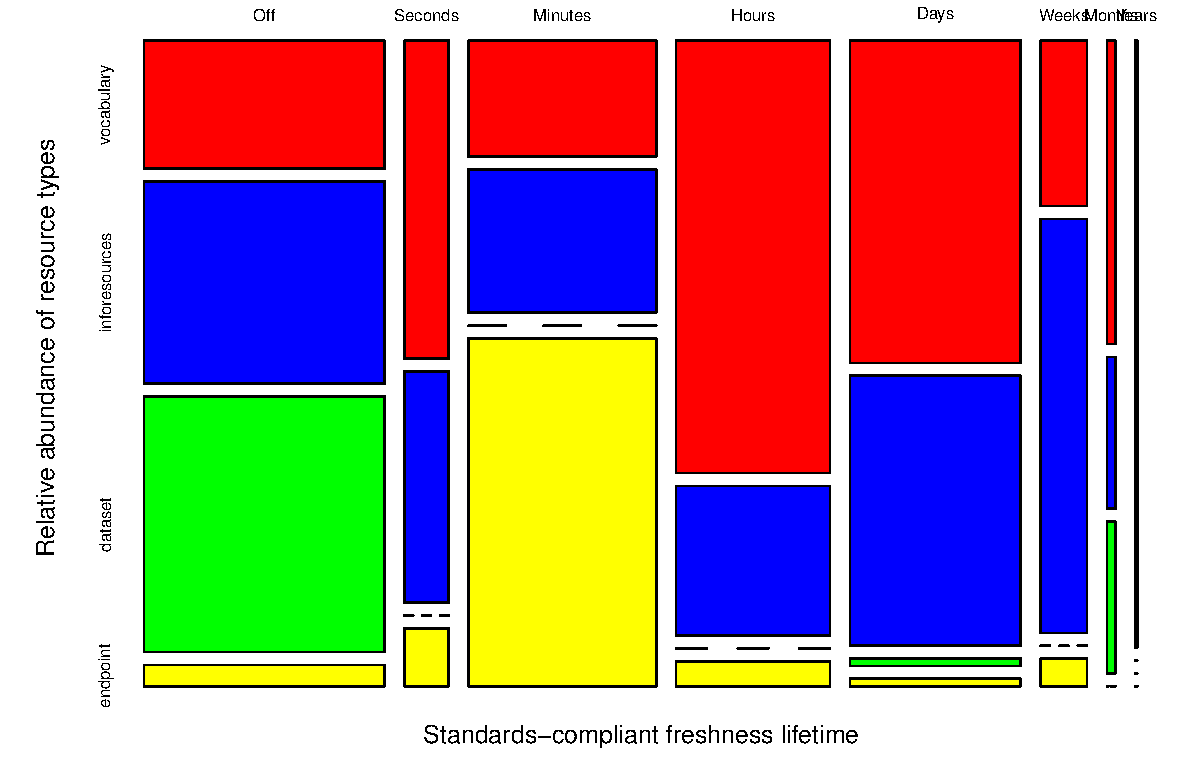
\includegraphics[width=.9\textwidth]{hardtable.pdf}}
  \caption{Mosaic Plot. On the vertical axis, the size of the boxes
    are determined by the fraction of the types of resources. On the
    horizontal axis the width of the boxes is proportional to the
    total counts, using the same bins as in
    Figure~\ref{fig:hardall}. Yellow boxes denote SPARQL Endpoints,
    green dataset descriptions, blue generic information resources and
    red vocabularies.}
  \label{fig:hardtable}
\end{figure}


We also note that prohibition of SPARQL results caching is rare,
amongst the servers that expose caching headers, it is common
that the result may be cached for some minutes.

\subsubsection{Simple heuristic freshness estimates}\label{sec:simplefresh}

We next consider the simple heuristic freshness lifetime as suggested
RFC7234, Section~4.2.2 and mentioned in the introduction.

\begin{figure}[th!]
  \centerline{%
    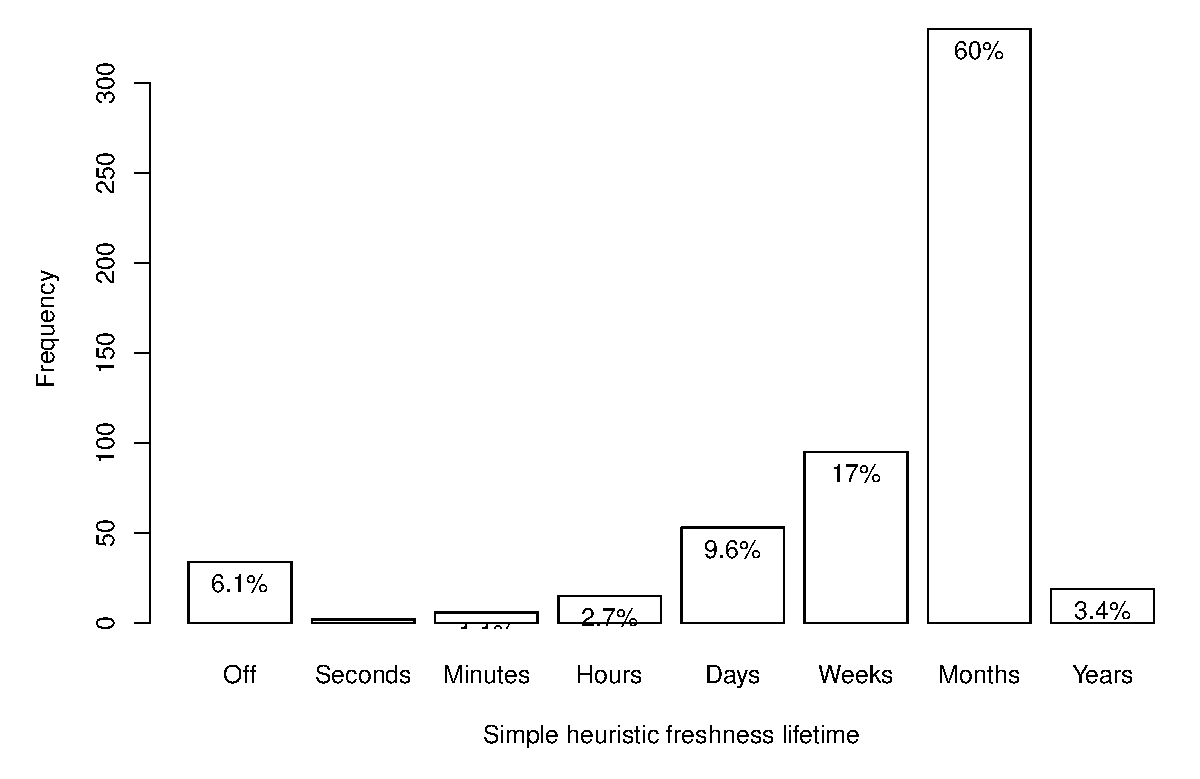
\includegraphics[width=.9\textwidth]{heuristicall.pdf}}
  \caption{Barplot counting all simple heuristic freshness lifetimes
    found. Bins as in Figure~\ref{fig:hardall}.}
  \label{fig:heuristicall}
\end{figure}

We were able to compute a heuristic lifetime for 554 resources, a
larger number than standards-compliant resources. In
Figure~\ref{fig:heuristicall}, we see that the distribution of
lifetimes are radically different from the case in
Figure~\ref{fig:hardall}. In this case, we may cache many resources
for months. Only a handful of resources had changed in the last
minutes. Since this is based on actual times since last modifications,
this suggests that many resources should have had explicit cache
headers with very long lifetimes. This is supported by
DyLDO\cite{dyldo2}, which concludes that:
\begin{quote}
[\ldots] We found that 62.2\% of documents didn’t change over the six
months and found that 51.9\% of domains were considered static.
\end{quote}
This agrees well with that 60\% of the simple heuristic lifetimes are
in the month range. 

Moreover, by inspecting Figure~\ref{fig:heuristictable}, we
note that the difference between different types of resources is much
smaller. This is confirmed by a $\chi^2$ test that yields \pvalue =
0.02.

\begin{figure}[hb!]
  \centerline{%
    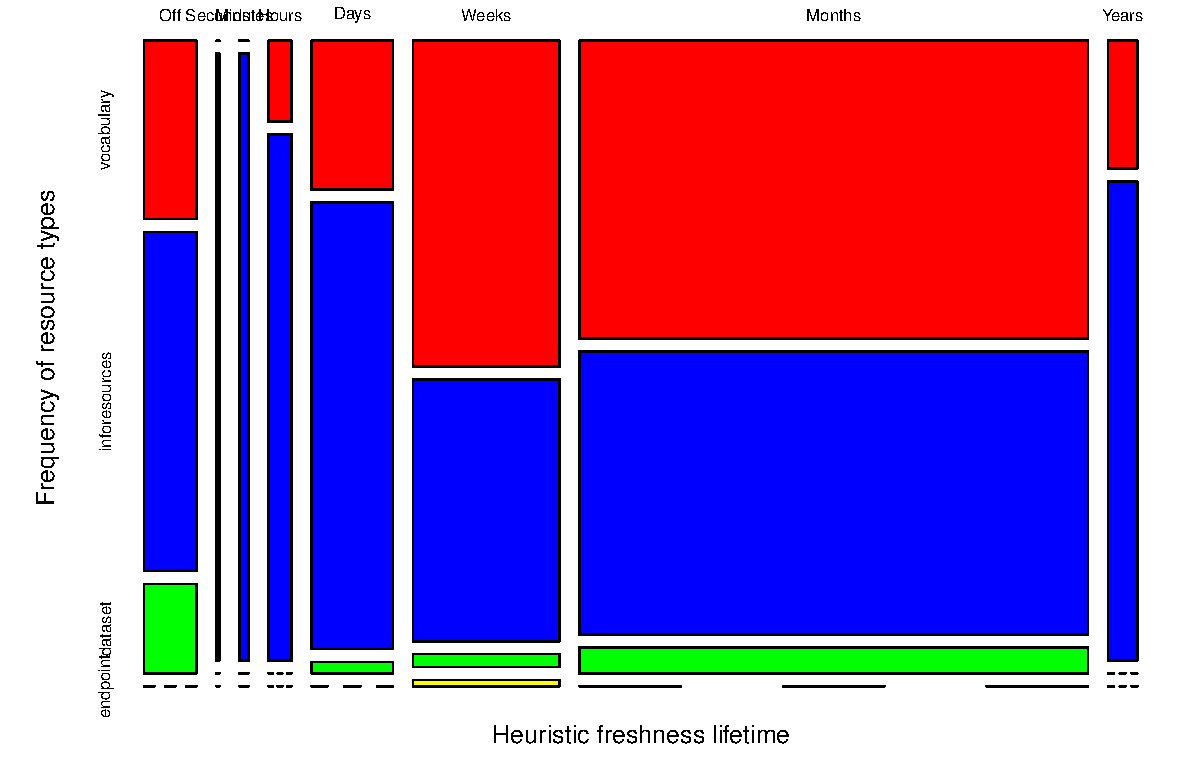
\includegraphics[width=.9\textwidth]{heuristictable.pdf}}
  \caption{Mosaic Plot for heuristic freshness lifetime. See caption
    of Figure~\ref{fig:hardtable} for description.  }
  \label{fig:heuristictable}
\end{figure}


We find that only one SPARQL Endpoint yields a heuristic lifetime, on
closer inspection, we find this to be hosted by
Dydra\footnote{http://dydra.com/}. We speculate that this is due to
that few underlying DBMS systems help track modification times in a
way that can be used on a SPARQL result basis.

\subsubsection{Heuristic freshness from Dublin Core properties}

We noted that the Dublin Core Metadata terms vocabulary has a number
of predicates that may become useful in determining heuristic
freshness in the future, so we recorded any statements containing the
predicates \rdfterm{dct:date}, \rdfterm{dct:accrualPeriodicity},
\rdfterm{dct:created}, \rdfterm{dct:issued}, \rdfterm{dct:modified} or
\rdfterm{dct:valid}.

First, we compare dates given in \rdfterm{dct:modified} to dates given
in \httph{Last-Modified} when both are available for a resource. They
are often not the same, but it appears that dates in the former are
further back in time than the latter. We speculate that this may be
due to that the web-server tracks semantically insignificant changes
through the file system, while authors of RDF only update timestamp
when significant changes are made, or it may be that authors forget to
update their timestamps.

\rdfterm{dct:modified} occurs in 2687 triples, but 2487 of these does
not have the Request-URI of the information resource as their subject,
i.e. it gives the last modification time of some subgraph of the
returned RDF. Nevertheless, given its prevalence, it is highly likely
that the presence of \rdfterm{dct:modified} will be useful in
determining a heuristic freshness lifetime, as the latest date may be
used.

\rdfterm{dct:valid} occurred 21 times, and could be used in lieu of an
\httph{Expires} header, but none of these occurrences had a date in the
future.

\rdfterm{dct:accrualPeriodicity} occurred only twice, and in neither
case contained machine readable data.

\rdfterm{dct:date}, \rdfterm{dct:created} and \rdfterm{dct:issued}
were present in 36, 389 and 1475 triples respectively. They correspond
roughly to the \httph{Date} header, which is present in all requests,
and they are therefore not important, but given their prevalence they
could be useful in further analysis.

\subsection{Cache validation}

Hitherto, we have considered the case where the client or proxy does
not send a HTTP request to the server when a resource that is present
in the cache is requested. This is desirable if the client can be
sufficiently confident that the response is fresh, either by having a
standards-compliant freshness lifetime or a heuristic to determine
it. At the end of this period, or if the previous response had no
lifetime, due to lack of information, or to that the server has stated
so in the \httph{Cache-Control} header, responses must be
revalidated. In this case, RFC7232 defines the behaviour, with
\httph{ETag} and \httph{Last-Modified} as the relevant response
headers.

The BTC had recorded these headers in their data, where 1733 had the
\httph{ETag} header and 690 had \httph{Last-Modified} with a great
overlap. For the resources where either or both were available, we
made our initial request conditional, and 911 responses were verified
as still fresh. 

In total, 1260 successful initial responses contained
an \httph{ETag}, 606 for vocabularies, 117 for datasets, just 12 for
endpoints and 525 for unclassified information resources.

To see if the server actually supported conditional requests, and not
just merely set the response headers, we made another 1822 requests to
the resources that had these headers. Then, we checked if the response
code was 200, and the conditional headers had not changed since our
initial requests. In 85 cases, conditional requests were not supported
according to the standard, no cases for endpoints, 3 for datasets and
23 for vocabularies, 59 for generic information resources.

\section{Conclusions and outlook}

We found moderate uptake for HTTP caching and conditional requests in
the Semantic Web. We found, in agreement with DyLDO\cite{dyldo2}, that
many resources change at a very slow pace, but also that this is not
reflected in the standards-compliant freshness lifetimes advertized by
servers.

We found that errors are commonplace, but that they does not usually
pertain to the caching headers. We found a small number of
self-contradictory \httph{Cache-Control} headers, and some servers
that set conditional request response headers, that could not support
conditional requests.

It is possible in a substantial number of cases to compute a heuristic
freshness lifetime, either from the \httph{Last-Modified} header, or
from Dublin Core properties. 

For SPARQL endpoints, we found that conditional requests are 
seldomly supported, but standards-compliant freshness lifetimes have
been seen, and since it is supported by DBPedia, benefits from caching
may be realized already.

In spite of this, most of the Semantic Web is unhelpful in spite of
being slowly changing.

\subsection{Future work}

In this work, we have only explored the cases where the server is
cooperative, in the sense that message data or metadata provides at
least a hint of a resource's cacheability. We also noted that the
majority of the Semantic Web is unhelpful. Therefore, an interesting
direction is to learn the change frequency of resources to use in a
heuristic freshness lifetime estimation. However, such work should
operate within the loose constraints of RFC7234, Section~4.2.2, and
should find it niche when the other techniques described in this paper
are unavailable. Once this is done, the correctness of caching headers
should be assessed, possibly using contigency tables.

Investigate whether curated collections such as LOV or SPARQLES
contain resources that has different characteristics. Since the
different sources we surveyed overlap, this cannot be done with
Pearson's $\chi^2$ test, but requires more sophisticated statistics.

We found that some implementations are likely better than others, but
further understanding of these differences are impeded by the fact
that most \httph{Server} headers contained very little
information. Future work could seek more sophisticated fingerprinting
and understanding of the nature of these differences.

Further investigate the suitability of the \rdfterm{dct:modified}
property for estimating heuristic freshness.

Estimating the freshness lifetime is a challenging problem for data
owners. It must necessarily involve the human users involved in the
publishing cycle since they are making a committment about future
changes. Designing user support systems as well as interfaces that fit
the publisher's workflow, is an important problem.

For SPARQL Endpoints, it is interesting to examine the queries in a
shared proxy, e.g. an institutional cache or a Content
Delivery Network for frequent subpatterns, and prefetch and cache such
intermediate results so that subsequent queries can be answered in
part by the proxy.

Even though it is clear that other parts of the Web benefit greatly
from caching, and that the potential for HTTP metadata to better
reflect actual update practices in the Semantic Web is great,
estimating the actual impact of doing so should be done.

\subsection{Recommendations}

Based on the results of DyLDO, it is highly likely that most cache
prohibitions are misguided, and server administrators are advised to
turn them off unless they are sure they are required.

In many cases, setting a reasonable cache headers is straightforward,
and should be done by data owners. Framework authors should make it
easy to set the expected lifetime, heeding the metadata association
good practice recommendation of \cite{Jacobs:04:AWW}. If the author is
unable to influence HTTP headers, they should set a
\rdfterm{dct:valid} time into the future and make use of
\rdfterm{dct:modified}.

To allow generation and validation of \httph{Last-Modified} and
\httph{ETag} headers, DBMS authors should make sure it is much cheaper
to retrieve the modification time of any subgraph, than to retrieve
the subgraph itself. This would be a great improvement for
RFC7232-based caching, when revalidation is required. It would also
help simple heuristics based caching. Research in that direction has
been published in \cite{kaseicache}.

A change periodicity predicate should be standardized in VoID.

All Web cache implementations we have studied have cached responses in
the form of a key that identifies a serialized object. For short-term
impact, future work should accept this as an architectural constraint.

\paragraph*{Acknowledgements} The author would like to thank Jürgen
Umbrich and Martin Giese for careful review and critical comments, and
Gregory Todd Williams for promptly solving issues in the underlying
libraries used in this study, and Axel Polleres for encouraging comments.

\bibliographystyle{plain}
%\bibliographystyle{abbrv}
%\bibliographystyle{jbact}
%\bibliographystyle{splncs03}
\bibliography{webarch,data,rfc,hypermedia,dynamicity,stat1,specs,vocabs}


\begin{subappendices}
\renewcommand{\thesection}{\Alph{section}}%

\section{Implementation of data reduction}\label{app:reduction}

The Billion Triple Challenge 2014 dataset provided data in the form of
NQuad files. Due to the presence of invalid RDF, we iterated through
the NQuad files on a line-by-line basis. First, we matched each line
against a regular expression were lines matching
\texttt{ontology|endpoint|sparql|vocabular} passed the filter. Then,
the Perl framework
RDF::Trine\footnote{https://metacpan.org/release/GWILLIAMS/RDF-Trine-1.011}
was used to parse the line. Lines that failed to parse were
discarded. We have not investigated whether this could introduce
biases. Statements were then accepted into a new NQuad file if they
had a predicate that matched the \rdfterm{sd:endpoint} or matched a
case-insensitive regular expression \texttt{sparql} if the subject and
objects were both resources, or the predicates
\rdfterm{void:vocabulary}, \rdfterm{rdfa:vocabulary}, or
\rdfterm{api:vocabulary}, as well as having a resource as
object. Finally, statements with the the classes
\rdfterm{cogs:Endpoint}, \rdfterm{owl:Ontology} and
\rdfterm{voaf:Vocabulary} in the object position were also
accepted\footnote{LOV may be used to resolve these prefixed
  names}. More classes and properties were considered, but not used in
the data reduction if they did not occur in the original data.

In the next step, we filtered out statements with URIs that were
invalid or irrelevant, e.g. URIs that didn't have a scheme or where
the scheme wasn't HTTP(S), or they were referring to private IP addresses.

We then sought to classify resources into the categories ``endpoint''
for SPARQL endpoints, ``vocabulary'' for vocabularies, ``dataset'' for
datasets that may contain further descriptions of several resources,
or simply ``inforesources'' for those that did not fit in the above
classes. To do so, we classified based on certain predicates and
classes. Additionally, URIs derived from prefix.cc were classified as
``vocabulary'' (even if we found several that were not) and those from
SPARQLES as ``endpoint''.

Since we blatantly violated URI opacity with our regular expression
matching in the first step, we needed to further filter candidates for
SPARQL endpoints. This step therefore included filtering as well as
classification.

We found in the data a large number of ontologies that consist of many
information resources with just a few triples in each. Since they
appear to be produced by the same software, usually Semantic
Mediawiki, we assume that they are configured with a single setup, and
thus we will merely sample these resources.

We continued to also sample the HTTP headers gathered in the BTC2014
dataset. 
%as they had recorded some of the relevant headers,
%\httph{Expires}, \httph{Last-Modified} and \httph{ETag}. 
First, we traversed the files with a simple UNIX \texttt{grep} to find
the resources that had reported one of the RDF serializations as
content type. We then traversed this list, first discarded the
resources that did not have a valid IRI (this amounted to just 3273
resources). For the resources we found, as well as for the resources
that was of \rdfterm{rdf:type owl:Ontology} above, we kept one
resource per hostname, with the exception of the popular blogging
platforms Livejournal and SAPO, where each blog has their own host and
they expose FOAF data. For those, we only kept one hostname. 

\section{Implementation of spider}\label{app:fetcher}

We then developed a fairly elaborate parallel spider to examine the
resources found on hosts that the previous steps deemed interesting
using the Perl frameworks RDF::Trine and libwww. The spider operated
with a timeout of 20 seconds and a maximum message size it would
accept of 1 MB.

The parallel spider would then launch a process per host, but each
request to one host would be delayed by 10 seconds. For each host, the
spider would go through the list of URLs found by previous steps for
that host. Since the BTC2014 recorded the \httph{Expires},
\httph{Last-Modified} and \httph{ETag} headers where they existed, we
first examined if any of the resources were still fresh, but none
were. Wherever the last two headers existed, we added the
corresponding \httph{If-Modified-Since} and \httph{If-None-Match}
headers for a conditional initial request.

\begin{table}
\caption{Recorded HTTP headers}\label{tab:headers}
 \begin{tabular}{ | l |  p{1.4cm} | p{6.8cm} |}
    \hline
    Header & Reference & Description \\ \hline
\httph{Age} & RFC7234 & When obtaining response from a cache, the number of
seconds since validation \\ \hline
\httph{Cache-Control} & RFC7234 & Header used for a variety of directives \\ \hline
\httph{Expires} & RFC7234  & Gives the date/time after which the
   response is considered stale. \\ \hline
\httph{Pragma} & RFC7234 & Archaic HTTP 1.0 header  \\ \hline
\httph{Warning} & RFC7234  & For additional information about possible incorrectness \\ \hline
\httph{Content-Type} & RFC7231 & To select the correct parser \\ \hline
\httph{If-None-Match} & RFC7232  & Request header to check if
                                   \httph{ETag} has changed   \\ \hline
\httph{If-Modified-Since} & RFC7232  & Request header to check if
                                   \httph{Last-Modified} has changed    \\ \hline
\httph{Last-Modified} & RFC7232 & When the resource was last modified \\ \hline
\httph{ETag} & RFC7232 & An opaque validator to check if the resource
has changed  \\ \hline
\httph{X-Cache} &  & Inserted by some caches to indicate cache status \\ \hline
\httph{Date} & RFC7231 & The time of the message. Used in conditional requests
and heuristics \\ \hline
\httph{Surrogates} & Edge \cite{edgearch} & Draft
to allow fine-grained control for proxies. \\ \hline
\httph{Client-Aborted} & libwww  & Header inserted by User
Agent to indicate that it aborted the download \\ \hline
\httph{Client-Warning} & libwww  & Header inserted by User
Agent to give details about problems with the download \\ \hline

    \hline
    \end{tabular}
\end{table}


For endpoints, we made the following SPARQL query:
\begin{verbatim}
SELECT DISTINCT ?Concept WHERE {[] a ?Concept} LIMIT 2
\end{verbatim}
which should be quite light, yet likely yield results.

Then, the first request would be made, and a selection of the
resulting HTTP headers recorded in an per-host NQuads file. For this
purpose, we developed and released a module
RDF::Generator::HTTP\footnote{https://metacpan.org/release/KJETILK/RDF-Generator-HTTP-0.003}
to the Comprehensive Perl Archive Network. We recorded whether the
conditional request showed that the BTC data were still fresh, and if
it was, we retrieved the current data, as we had not coupled the
headers to the body in our original retrieval.

Based on the resulting headers, we let
libwww\footnote{https://metacpan.org/release/GAAS/libwww-perl-6.04}
calculate both standards-compliant and simple heuristic freshness
lifetime.

If the initial response had RFC7232 headers, we make another
request to see if the server just included the headers but does not
actually support conditional requests. The heuristic we employed is
that if the headers remain the same, but the result was returned,
rather than just a response code \httph{304} (which indicates that the
previous result can be reused), then the server does most probably not
support it.

For endpoints, we examined the response message, to see if there are
any results to our query, and recorded that if there are. In addition
to the endpoints registered in the SPARQLES survey, our process found
18~endpoints that responded with results.

For all others, we parsed the response, and recorded any errors if the
parser concluded the content were invalid.

For resource types other than ``vocabulary'', we look for SPARQL
endpoints in the response, using the predicates \rdfterm{sd:endpoint}
and \rdfterm{void:sparqlEndpoint}. We then do the same query as above
and record the relevant headers. Unfortunately, we found early that
this only turns up misconfigured endpoints that point to localhost,
and was removed from the spider for the final analysis.

Finally, if the LOV SPARQL endpoint used a URI for the vocabulary that
was different from the namespace URI (after a normalization step),
another request would be made to record the selected HTTP headers from
that as well.

\section{Statistical method}\label{app:stats}

The hypothesis tests in this paper is implemented using \emph{contigency
  tables} (see e.g. \cite{kn:bj}). This formalism is suited to see if the
distribution of  \httph{Server} headers are different for those implementations that
offer caching headers from those that don't. Intuitively, we expect
these distributions to be similar, ``long-tail'' distributions, i.e. a
handful of servers are used by a large number of projects, and then it
falls off rapidly, and so, some servers are used only by very
few. Likewise, it is to be expected that only a few projects have
given caching enough attention, but that they account for the majority
of the support. The question is if the presence of caching headers is
merely a matter of proportion, or if there are some that have given it
more attention, but still is in relatively little use.

Using the statistics system R\cite{kn:r}, we use a statistical test,
namely Pearson's $\chi^2$ test with simulated \pvalue (based on 10000
replicates). The simulation is done using a Monte Carlo method to
compensate for the fact that many servers will not expose caching
headers at all, an issue that would otherwise violate the underlying
assumptions of the test.

\end{subappendices}



\end{document}
